\chapter{Results}

\section{Hyper-Parameter Optimization}

    In order to significantly reduce the cost of evaluation (re-training
    the whole model from scratch with a different set of hyper-parameters),
    the training set used for hyper-parameter tuning has been
    limited to the PSICOV150 families.
    Hyperopt stopped after only 32 iterations with a maximum of 48,9 \%
    of best-L PPV on the 30 validation proteins.

    \begin{figure}[H]
        \begin{center}
            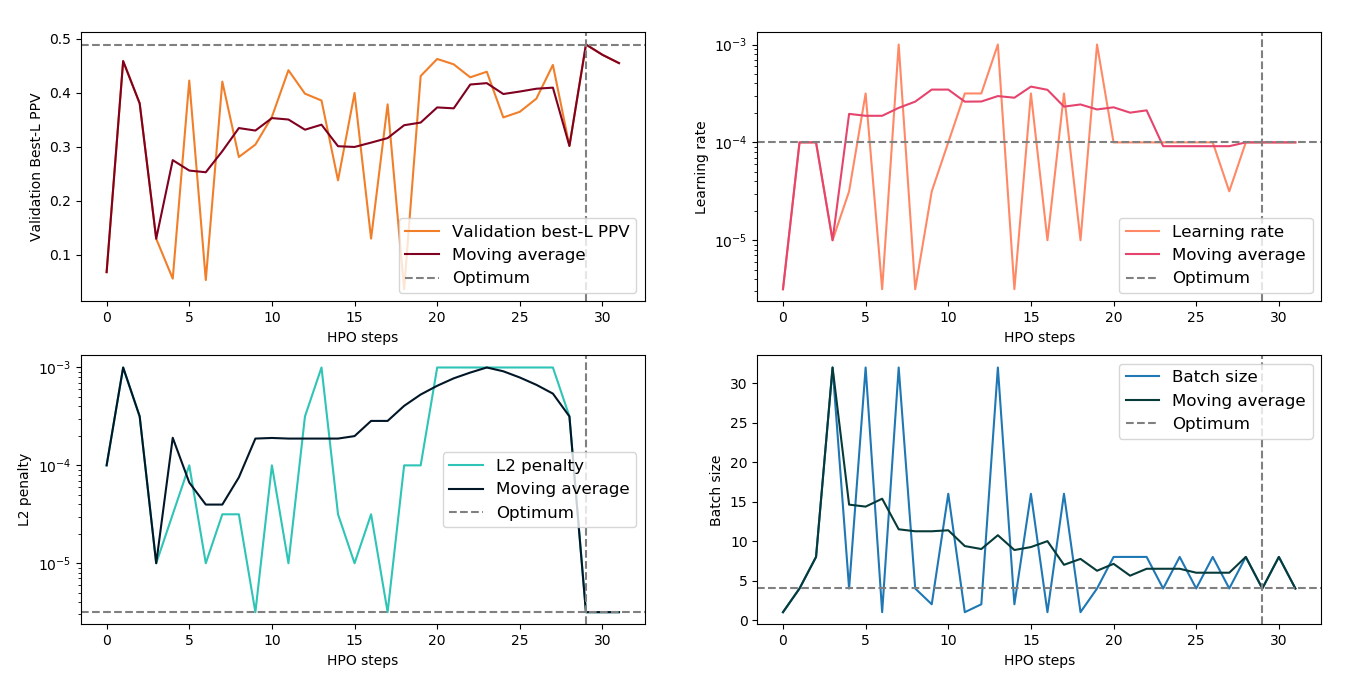
\includegraphics[width=\textwidth, keepaspectratio]{imgs/hpo.png}
            \caption{Performance and hyper-parameter values as a function of the number
            of Hyper-Parameter Optimization (HPO) iterations.
            Top left figure illustrates the optimal point whose value on x-axis
            is given by the HPO iteration that yields highest validation Best-L PPV.
            Optimal values for the learning rate, L2 penalty and batch size are denoted
            by dashed lines in top right, bottom left and bottom right figures, respectively.}
            \label{hpoparams}
        \end{center}
    \end{figure}

    As can be observed in top left figure in \ref{hpoparams}, a high-quality solution (local maximum)
    was found in the very first iterations, but the algorithm continued to explore and
    found its best solution after 30 iterations with a completely different set of parameters:
    L2 regularization parameter changed from $10^{-3}$ to $\frac{1}{2} 10^-{5}$ and
    batch size changed from $32$ proteins to only $4$. Because these two solutions
    are very distant in the hyper-parameter space and have similar performance,
    it can be suggested that the latter is the search space is multimodal.

    \begin{figure}[H]
        \begin{center}
            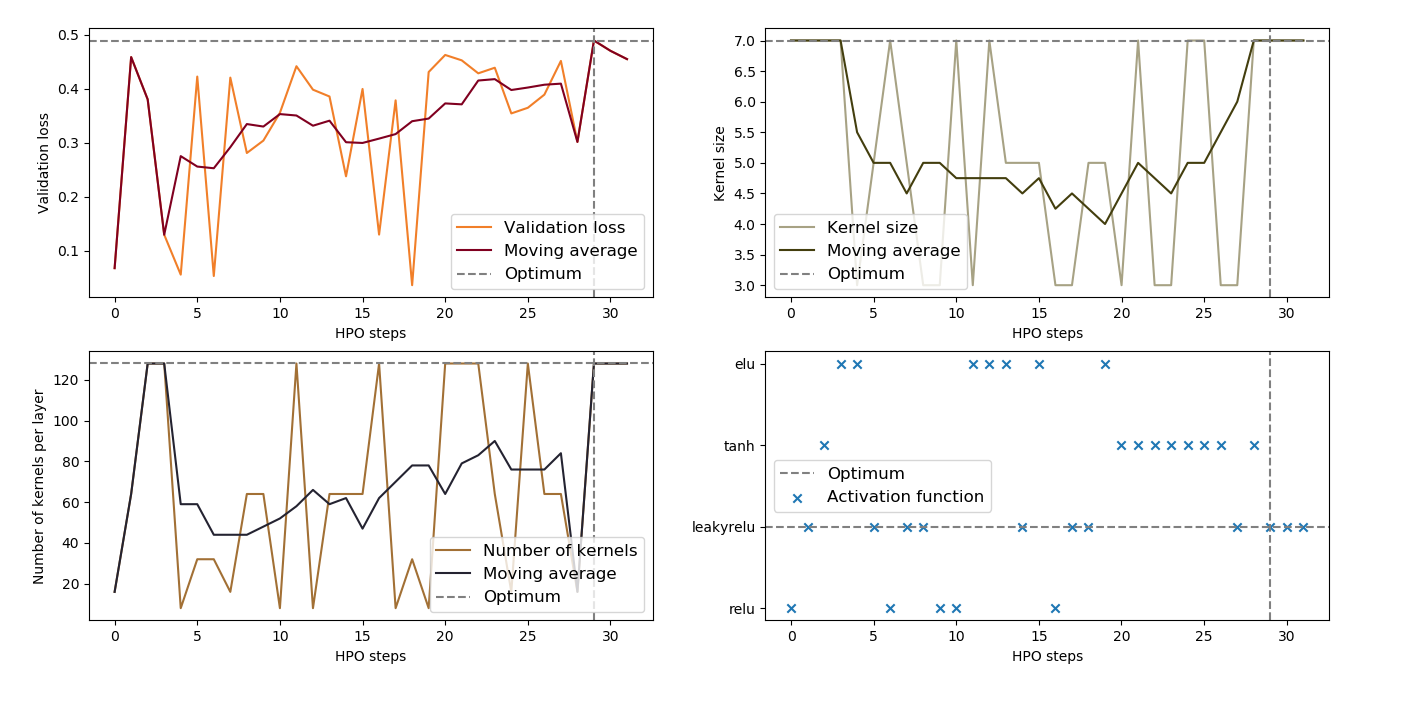
\includegraphics[width=\textwidth, keepaspectratio]{imgs/hpo2.png}
            \caption{Performance and hyper-parameter values as a function of the number
            of Hyper-Parameter Optimization (HPO) iterations.
            Top left figure illustrates the optimal point whose value on x-axis
            is given by the HPO iteration that yields highest validation Best-L PPV.
            Optimal values for kernel size, number of kernels and activation function are denoted
            by dashed lines in top right, bottom left and bottom right figures, respectively.}
            \label{hpoparams2}
        \end{center}
    \end{figure}

    Optimal hyper-parameter values are provided in table \ref{besthp}.
    It turned out that batch normalization is required, which is consistent
    with the fact that a very large network depth has been found
    (3 + 18 + 18 layers). A batch size of 4 is sufficient, which makes sense
    since each example is a protein of size $L$ containing potentially
    $L (L - 1) / 2$ residue pairs and each residue pair is a statistical
    example \textit{per se}.

    \begin{table}[H]
        \centering
        \begin{tabular}{lll}
          \hline
          Module & Hyper-parameter & Set of values \\
          \hline
          \hline
          General & Batch size & $4$ \\
                  & Batch normalization & $\top$ \\
                  & Track running state & $\bot$ \\
                  & Learning rate & $10^{-4}$ \\
                  & L2 penalty & $10^{-4}$ \\
                  & Parameter optimization & $\text{Adam}$ \\
                  & Activation function & $\text{LeakyReLU}$ \\
                  & Use global modules & $\top$ \\
          \hline
          Global module & Depth & $3$ \\
          \hline
          1-dimensional module & Depth & $18$ \\
                               & Filter size & $7$ \\
                               & Number of filters & $128$ \\
          \hline
          2-dimensional module & Depth & $18$ \\
                               & Filter size & $7$ \\
                               & Number of filters & $128$ \\
          \hline
        \end{tabular}
        \captionof{table}{Set of hyper-parameter values obtained at optimal point.}
        \label{besthp}
    \end{table}

    A L2 regularization parameter of $10^{-4}$ has been found.
    However, this value has been replaced
    by $10^{-5}$ for training the final model on the whole training set since
    the latter contains much more proteins than PSICOV150 alone, alleviating
    the need for regularization.

    \begin{figure}[H]
        \begin{center}
            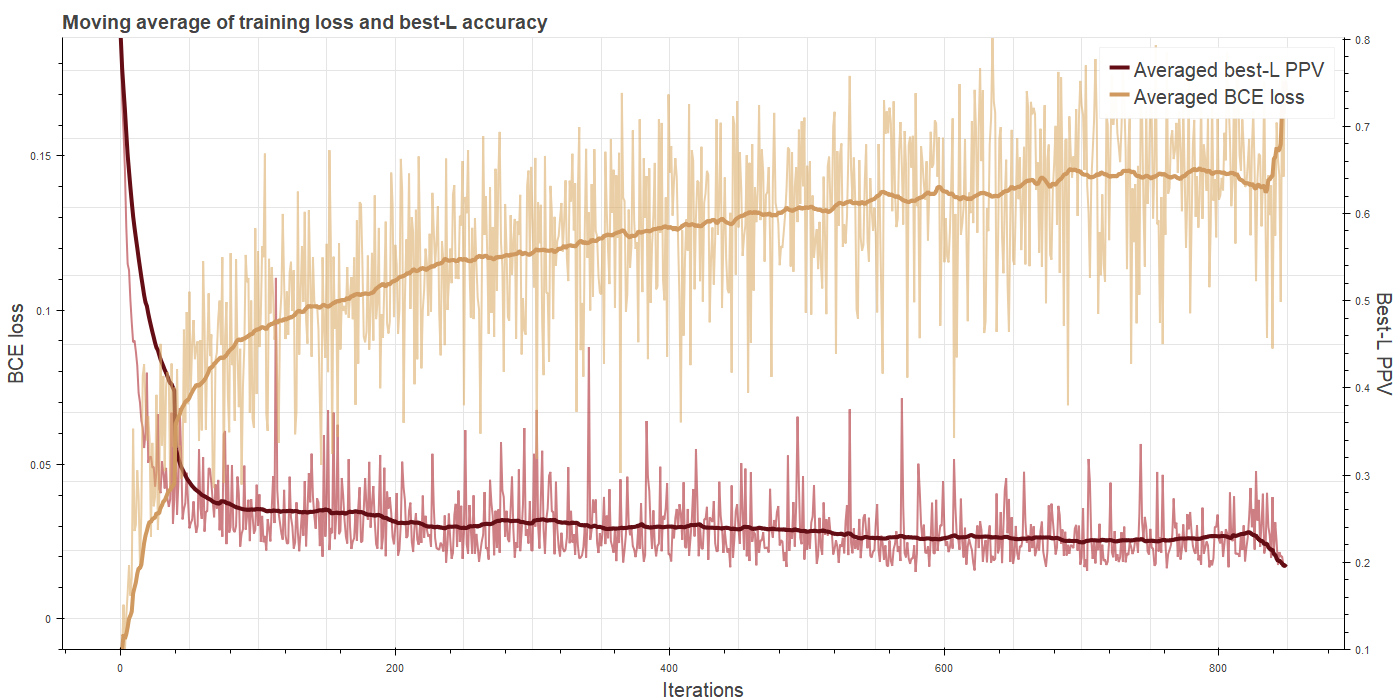
\includegraphics[width=\textwidth, keepaspectratio]{imgs/loss.png}
            \caption{Binary Cross-Entropy loss and best-L PPV computed on
              a rolling window of batches, related to the training phase of the model
              with best hyper-parameters.}
            \label{lossandppv}
        \end{center}
    \end{figure}

    Convergence of the final model on PSICOV150 is shown in figure~\ref{lossandppv}.
    It can be noticed that binary cross-entropy is directly and inversely
    related to the training PPV. The neural network takes approximately 850
    batches to converge. However, when trained on the whole training set, it takes
    approximately 16 000 batches and 4 days before the algorithm converges.

\section{Model evaluation on the different benchmark sets}

    Performance measured in table~\ref{benchmark} is the PPV obtained
    by only considering the top $L$ predicted probabilities as predicted
    contacts. In this way, the evaluation is based only on the contacts
    the predictive model is the most confident about.
    As can be observed, best-L PPV is significantly lower for short range contacts,
    regardless of the method used. Indeed, the number of residue pairs having a
    sequence separation between 6 \AA{} and 12 \AA{} is much smaller then for a
    separation between 12 \AA{} and 24 \AA{} (medium range) or above 24 \AA{} (long range).
    Short range best-L PPV is thus computed on the basis of much less confident
    predictions than in the other cases, making the evaluation much more disadvantageous.

    \begin{table}[H]
        \centering
        \resizebox{\textwidth}{!}{
        \begin{tabular}{|l|ccc|ccc|ccc|}
            \hline
            & & CASP11 & & & CAMEO & & & Membrane & \\
            \hline
            Method & Short & Medium & Long & Short & Medium & Long & Short & Medium & Long \\
            \hline
            \hline
            Proposed method & 0.24 & 0.28 & 0.37 & 0.21 & 0.24 & 0.26 & 0.12 & 0.17 & 0.30 \\
            RaptorX-Contact & 0.28 & 0.35 & 0.55 & 0.23 & 0.28 & 0.42 & 0.16 & 0.22 & 0.47 \\
            PconsC3         & 0.25 & 0.29 & 0.40 & 0.21 & 0.23 & 0.27 & 0.15 & 0.19 & 0.33 \\
            MetaPSICOV & 0.26 & 0.31 & 0.39 & 0.22 & 0.22 & 0.28 & 0.16 & 0.21 & 0.35 \\
            PlmDCA & 0.14 & 0.16 & 0.27 & 0.11 & 0.13 & 0.19 & 0.08 & 0.11 & 0.21 \\
            PSICOV & 0.14 & 0.15 & 0.24 & 0.13 & 0.14 & 0.18 & 0.09 & 0.11 & 0.20 \\
            mfDCA & 0.13 & 0.15 & 0.22 & 0.10 & 0.11 & 0.15 & 0.09 & 0.12 & 0.24 \\
            \hline
        \end{tabular}
        }
        \captionof{table}{Best-L PPV of different methods on short,
        medium and long-range contacts. Results are shown for the three
        different benchmark sets: CASP11 targets, CAMEO proteins, and
        the benchmark set of membrane proteins.}
        \label{benchmark}
    \end{table}

    Unsupervised methods (namely DCA and PSICOV) are clearly outperformed by other methods.
    % TODO

    \subsection{CASP11}

        \begin{table}[H]
            \centering
            \resizebox{\textwidth}{!}{
            \begin{tabular}{|l|cccc|cccc|cccc|}
                \hline
                Method & \multicolumn{4}{|c|}{Short range} & \multicolumn{4}{|c|}{Medium range} & \multicolumn{4}{|c|}{Long range} \\
                \hline
                & L/10 & L/5 & L/2 & L & L/10 & L/5 & L/2 & L & L/10 & L/5 & L/2 & L \\
                \hline
                \hline
                EVfold          & 0.25 & 0.21 & 0.15 & 0.12 & 0.33 & 0.27 & 0.19 & 0.13 & 0.37 & 0.33 & 0.25 & 0.19 \\
                PSICOV          & 0.29 & 0.23 & 0.15 & 0.12 & 0.34 & 0.27 & 0.18 & 0.13 & 0.38 & 0.33 & 0.25 & 0.19 \\
                plmDCA          & 0.35 & 0.28 & 0.17 & 0.12 & 0.40 & 0.32 & 0.21 & 0.14 & 0.43 & 0.39 & 0.31 & 0.23 \\
                Gremlin         & 0.32 & 0.26 & 0.17 & 0.12 & 0.39 & 0.31 & 0.21 & 0.14 & 0.42 & 0.38 & 0.30 & 0.23 \\
                CCMpred         & 0.35 & 0.27 & 0.17 & 0.12 & 0.40 & 0.31 & 0.21 & 0.14 & 0.44 & 0.40 & 0.31 & 0.23 \\
                MetaPSICOV      & 0.69 & 0.58 & 0.39 & 0.25 & 0.69 & 0.59 & 0.42 & 0.28 & 0.60 & 0.54 & 0.45 & 0.35 \\
                RaptorX-Contact & 0.82 & 0.70 & 0.46 & 0.28 & 0.85 & 0.76 & 0.55 & 0.35 & 0.81 & 0.77 & 0.68 & 0.55 \\
                Proposed method & 0.64 & 0.54 & 0.37 & 0.24 & 0.65 & 0.57 & 0.41 & 0.30 & 0.63 & 0.58 & 0.47 & 0.37 \\
                \hline
            \end{tabular}
            }
            \captionof{table}{Best-L PPV of different methods on the CASP11 targets with different values for L.}
            \label{casp11benchmark}
        \end{table}

    \subsection{CAMEO}

        \begin{table}[H]
            \centering
            \resizebox{\textwidth}{!}{
            \begin{tabular}{|l|cccc|cccc|cccc|}
                \hline
                Method & \multicolumn{4}{|c|}{Short range} & \multicolumn{4}{|c|}{Medium range} & \multicolumn{4}{|c|}{Long range} \\
                \hline
                & L/10 & L/5 & L/2 & L & L/10 & L/5 & L/2 & L & L/10 & L/5 & L/2 & L \\
                \hline
                \hline
                EVfold          & 0.17 & 0.13 & 0.11 & 0.09 & 0.23 & 0.19 & 0.13 & 0.10 & 0.25 & 0.22 & 0.17 & 0.13 \\
                PSICOV          & 0.20 & 0.15 & 0.11 & 0.08 & 0.24 & 0.19 & 0.13 & 0.09 & 0.25 & 0.23 & 0.18 & 0.13 \\
                plmDCA          & 0.22 & 0.16 & 0.11 & 0.09 & 0.27 & 0.22 & 0.14 & 0.10 & 0.30 & 0.26 & 0.20 & 0.15 \\
                Gremlin         & 0.23 & 0.18 & 0.12 & 0.09 & 0.27 & 0.22 & 0.14 & 0.10 & 0.30 & 0.26 & 0.20 & 0.15 \\
                CCMpred         & 0.21 & 0.17 & 0.11 & 0.08 & 0.27 & 0.22 & 0.14 & 0.10 & 0.31 & 0.26 & 0.20 & 0.15 \\
                MetaPSICOV      & 0.56 & 0.47 & 0.31 & 0.20 & 0.53 & 0.45 & 0.32 & 0.22 & 0.47 & 0.42 & 0.33 & 0.25 \\
                RaptorX-Contact & 0.67 & 0.57 & 0.37 & 0.23 & 0.69 & 0.61 & 0.42 & 0.28 & 0.69 & 0.65 & 0.55 & 0.42 \\
                Proposed method & 0.54 & 0.44 & 0.31 & 0.21 & 0.56 & 0.47 & 0.35 & 0.24 & 0.51 & 0.45 & 0.35 & 0.26 \\
                \hline
            \end{tabular}
            }
            \captionof{table}{Best-L PPV of different methods on the CAMEO targets with different values for L.}
            \label{cameobenchmark}
        \end{table}

    \subsection{Membrane proteins}

        \begin{table}[H]
            \centering
            \resizebox{\textwidth}{!}{
            \begin{tabular}{|l|cccc|cccc|cccc|}
                \hline
                Method & \multicolumn{4}{|c|}{Short range} & \multicolumn{4}{|c|}{Medium range} & \multicolumn{4}{|c|}{Long range} \\
                \hline
                & L/10 & L/5 & L/2 & L & L/10 & L/5 & L/2 & L & L/10 & L/5 & L/2 & L \\
                \hline
                \hline
                EVfold          & 0.16 & 0.13 & 0.09 & 0.07 & 0.28 & 0.22 & 0.13 & 0.09 & 0.44 & 0.37 & 0.26 & 0.18 \\
                PSICOV          & 0.22 & 0.16 & 0.10 & 0.07 & 0.29 & 0.21 & 0.13 & 0.09 & 0.42 & 0.34 & 0.23 & 0.16 \\
                plmDCA          & 0.27 & 0.19 & 0.11 & 0.08 & 0.36 & 0.26 & 0.15 & 0.10 & 0.52 & 0.45 & 0.31 & 0.21 \\
                Gremlin         & 0.26 & 0.18 & 0.11 & 0.08 & 0.35 & 0.25 & 0.14 & 0.09 & 0.51 & 0.42 & 0.29 & 0.20 \\
                CCMpred         & 0.27 & 0.19 & 0.11 & 0.07 & 0.37 & 0.26 & 0.15 & 0.10 & 0.52 & 0.45 & 0.32 & 0.21 \\
                MetaPSICOV      & 0.45 & 0.35 & 0.22 & 0.14 & 0.49 & 0.40 & 0.27 & 0.18 & 0.61 & 0.55 & 0.42 & 0.30 \\
                RaptorX-Contact & 0.60 & 0.46 & 0.27 & 0.16 & 0.66 & 0.53 & 0.33 & 0.22 & 0.78 & 0.73 & 0.62 & 0.47 \\
                Proposed method & 0.38 & 0.30 & 0.20 & 0.13 & 0.45 & 0.37 & 0.25 & 0.17 & 0.58 & 0.51 & 0.40 & 0.30 \\
                \hline
            \end{tabular}
            }
            \captionof{table}{Best-L PPV of different methods on 398 membrane proteins with different values for L.}
            \label{cameobenchmark}
        \end{table}

\section{Sensitivity to the number of homologous sequences}

    \begin{figure}[H]
        \begin{center}
            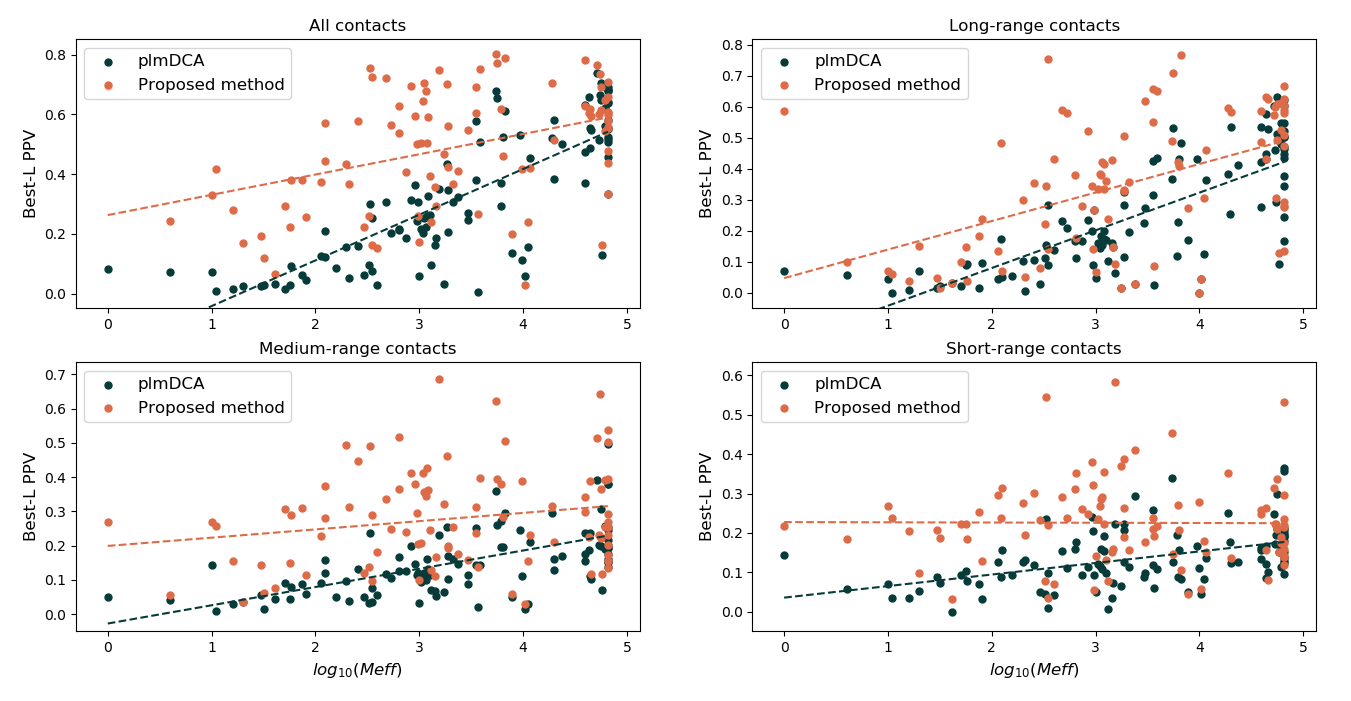
\includegraphics[width=\textwidth, keepaspectratio]{imgs/Meff.png}
            \caption{Performance as a function of the logarithm of the effective
            number of homologous sequences. Top figure shows the results on
            CASP11 targets for different types of contacts. Bottom left and bottom right figures
            focus on medium-range and long-range contacts, respectively.}
            \label{sensitivity}
        \end{center}
    \end{figure}

    \begin{figure}[H]
        \begin{center}
            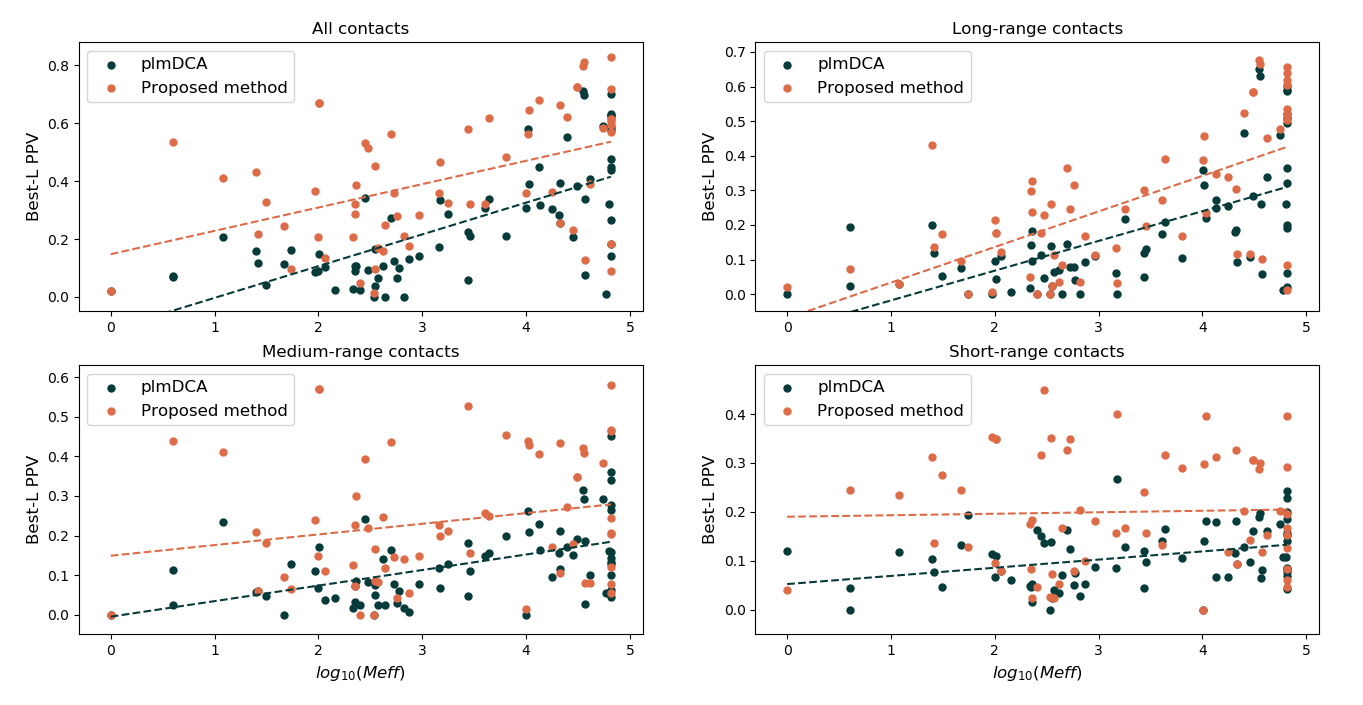
\includegraphics[width=\textwidth, keepaspectratio]{imgs/Meff_cameo.png}
            \caption{Performance as a function of the logarithm of the effective
            number of homologous sequences. Top figure shows the results on
            CAMEO targets for different types of contacts. Bottom left and bottom right figures
            focus on medium-range and long-range contacts, respectively.}
            \label{sensitivity}
        \end{center}
    \end{figure}

    \begin{figure}[H]
        \begin{center}
            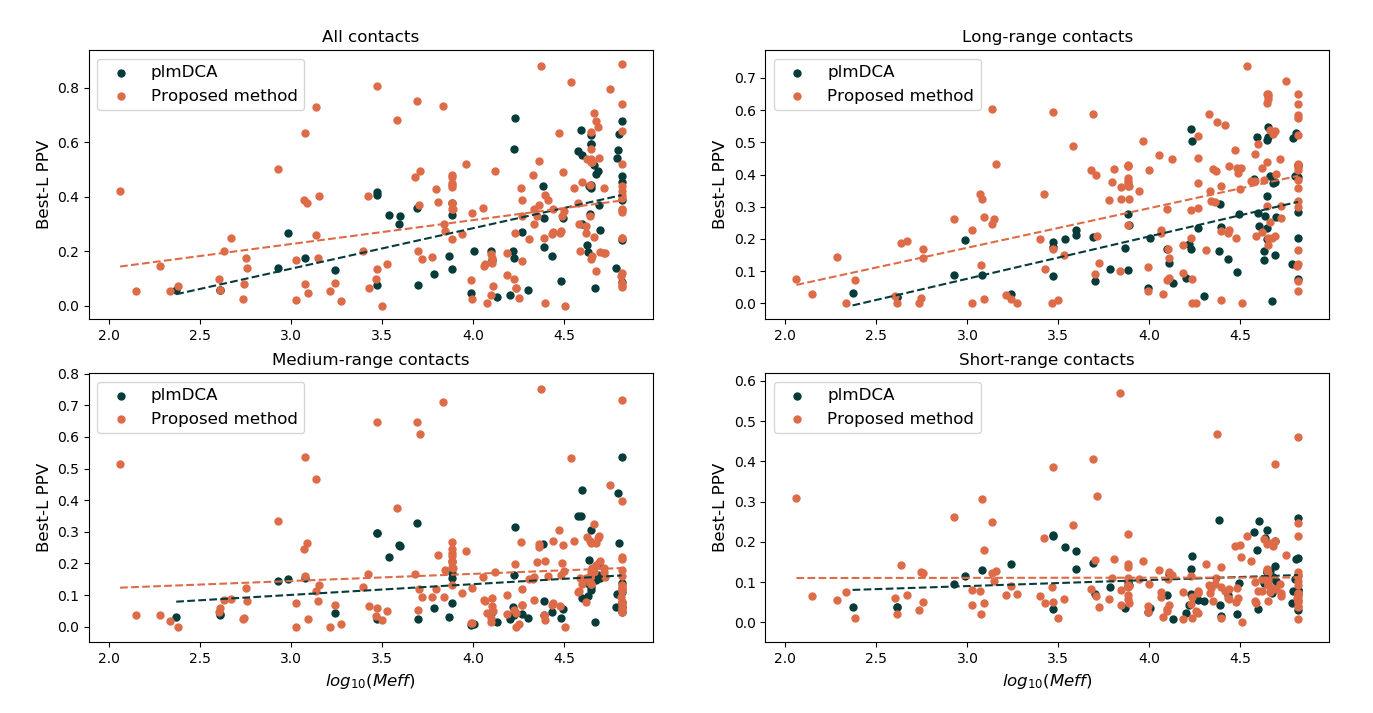
\includegraphics[width=\textwidth, keepaspectratio]{imgs/Meff_membrane.png}
            \caption{Performance as a function of the logarithm of the effective
            number of homologous sequences. Top figure shows the results on
            membrane proteins for different types of contacts. Bottom left and bottom right figures
            focus on medium-range and long-range contacts, respectively.}
            \label{sensitivity}
        \end{center}
    \end{figure}
